% 06-Resultados_Presentacion_Tesis.tex
% Diapositivas de la sección Resultados

\section{Resultados}

\begin{frame}
\frametitle{Evaluación de los Modelos}
\begin{itemize}
    \item Se evaluaron dos modelos principales: ResNet50 (CNN) y Vision Transformer (ViT).
    \item Ambos modelos fueron entrenados para detectar 15 patologías pulmonares, incluyendo COVID-19.
    \item Se utilizaron métricas como AUC-ROC, AUC-PR, F1-Score y Accuracy.
\end{itemize}
\end{frame}

\begin{frame}
\frametitle{Métricas de Evaluación}
\begin{itemize}
    \item \textbf{AUC-ROC}: Área bajo la curva ROC, mide la capacidad de discriminación del modelo.
    \item \textbf{AUC-PR}: Área bajo la curva Precisión-Recall, útil en clases desbalanceadas.
    \item \textbf{F1-Score}: Media armónica entre precisión y recall.
    \item \textbf{Accuracy}: Proporción de clasificaciones correctas.
\end{itemize}
\end{frame}

\begin{frame}
\frametitle{Comparativa de Resultados Globales}
\begin{itemize}
    \item Ambos modelos muestran resultados competitivos en la detección de patologías pulmonares.
    \item El modelo ViT destaca en la detección de COVID-19 y otras patologías complejas.
    \item ResNet50 mantiene un rendimiento robusto y eficiente en la mayoría de las clases.
\end{itemize}
\end{frame}

\begin{frame}
\frametitle{Resultados por Patología (AUC-ROC)}
\begin{figure}[ht!]
    \centering
    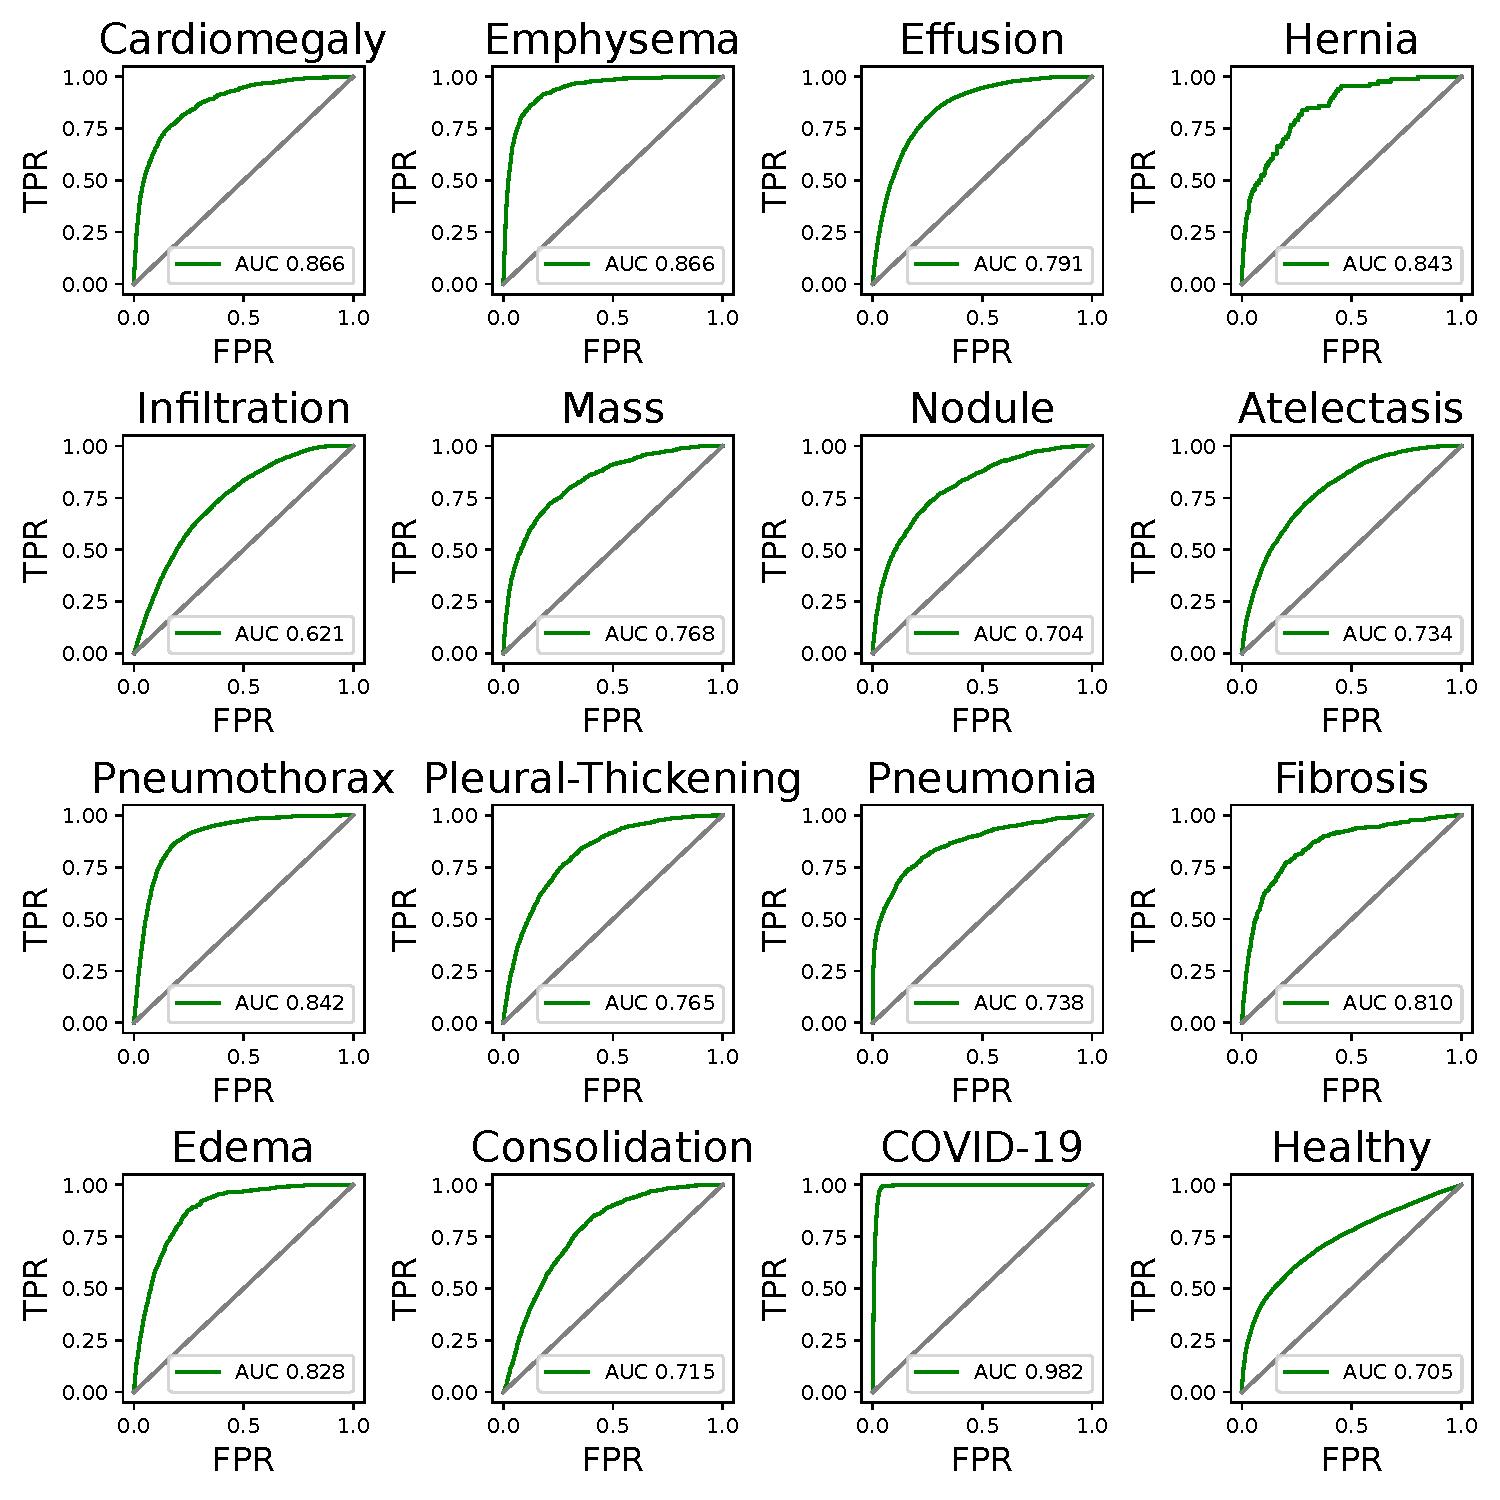
\includegraphics[width=0.9\textwidth]{../Chapters/4. ViT-Lung/images/ROC_AUC_ViT.pdf}
    \caption{Curvas ROC para las principales patologías detectadas por el modelo ViT.}
\end{figure}
\end{frame}

\begin{frame}
\frametitle{Visualización de la Atención del Modelo}
\begin{figure}[ht!]
    \centering
    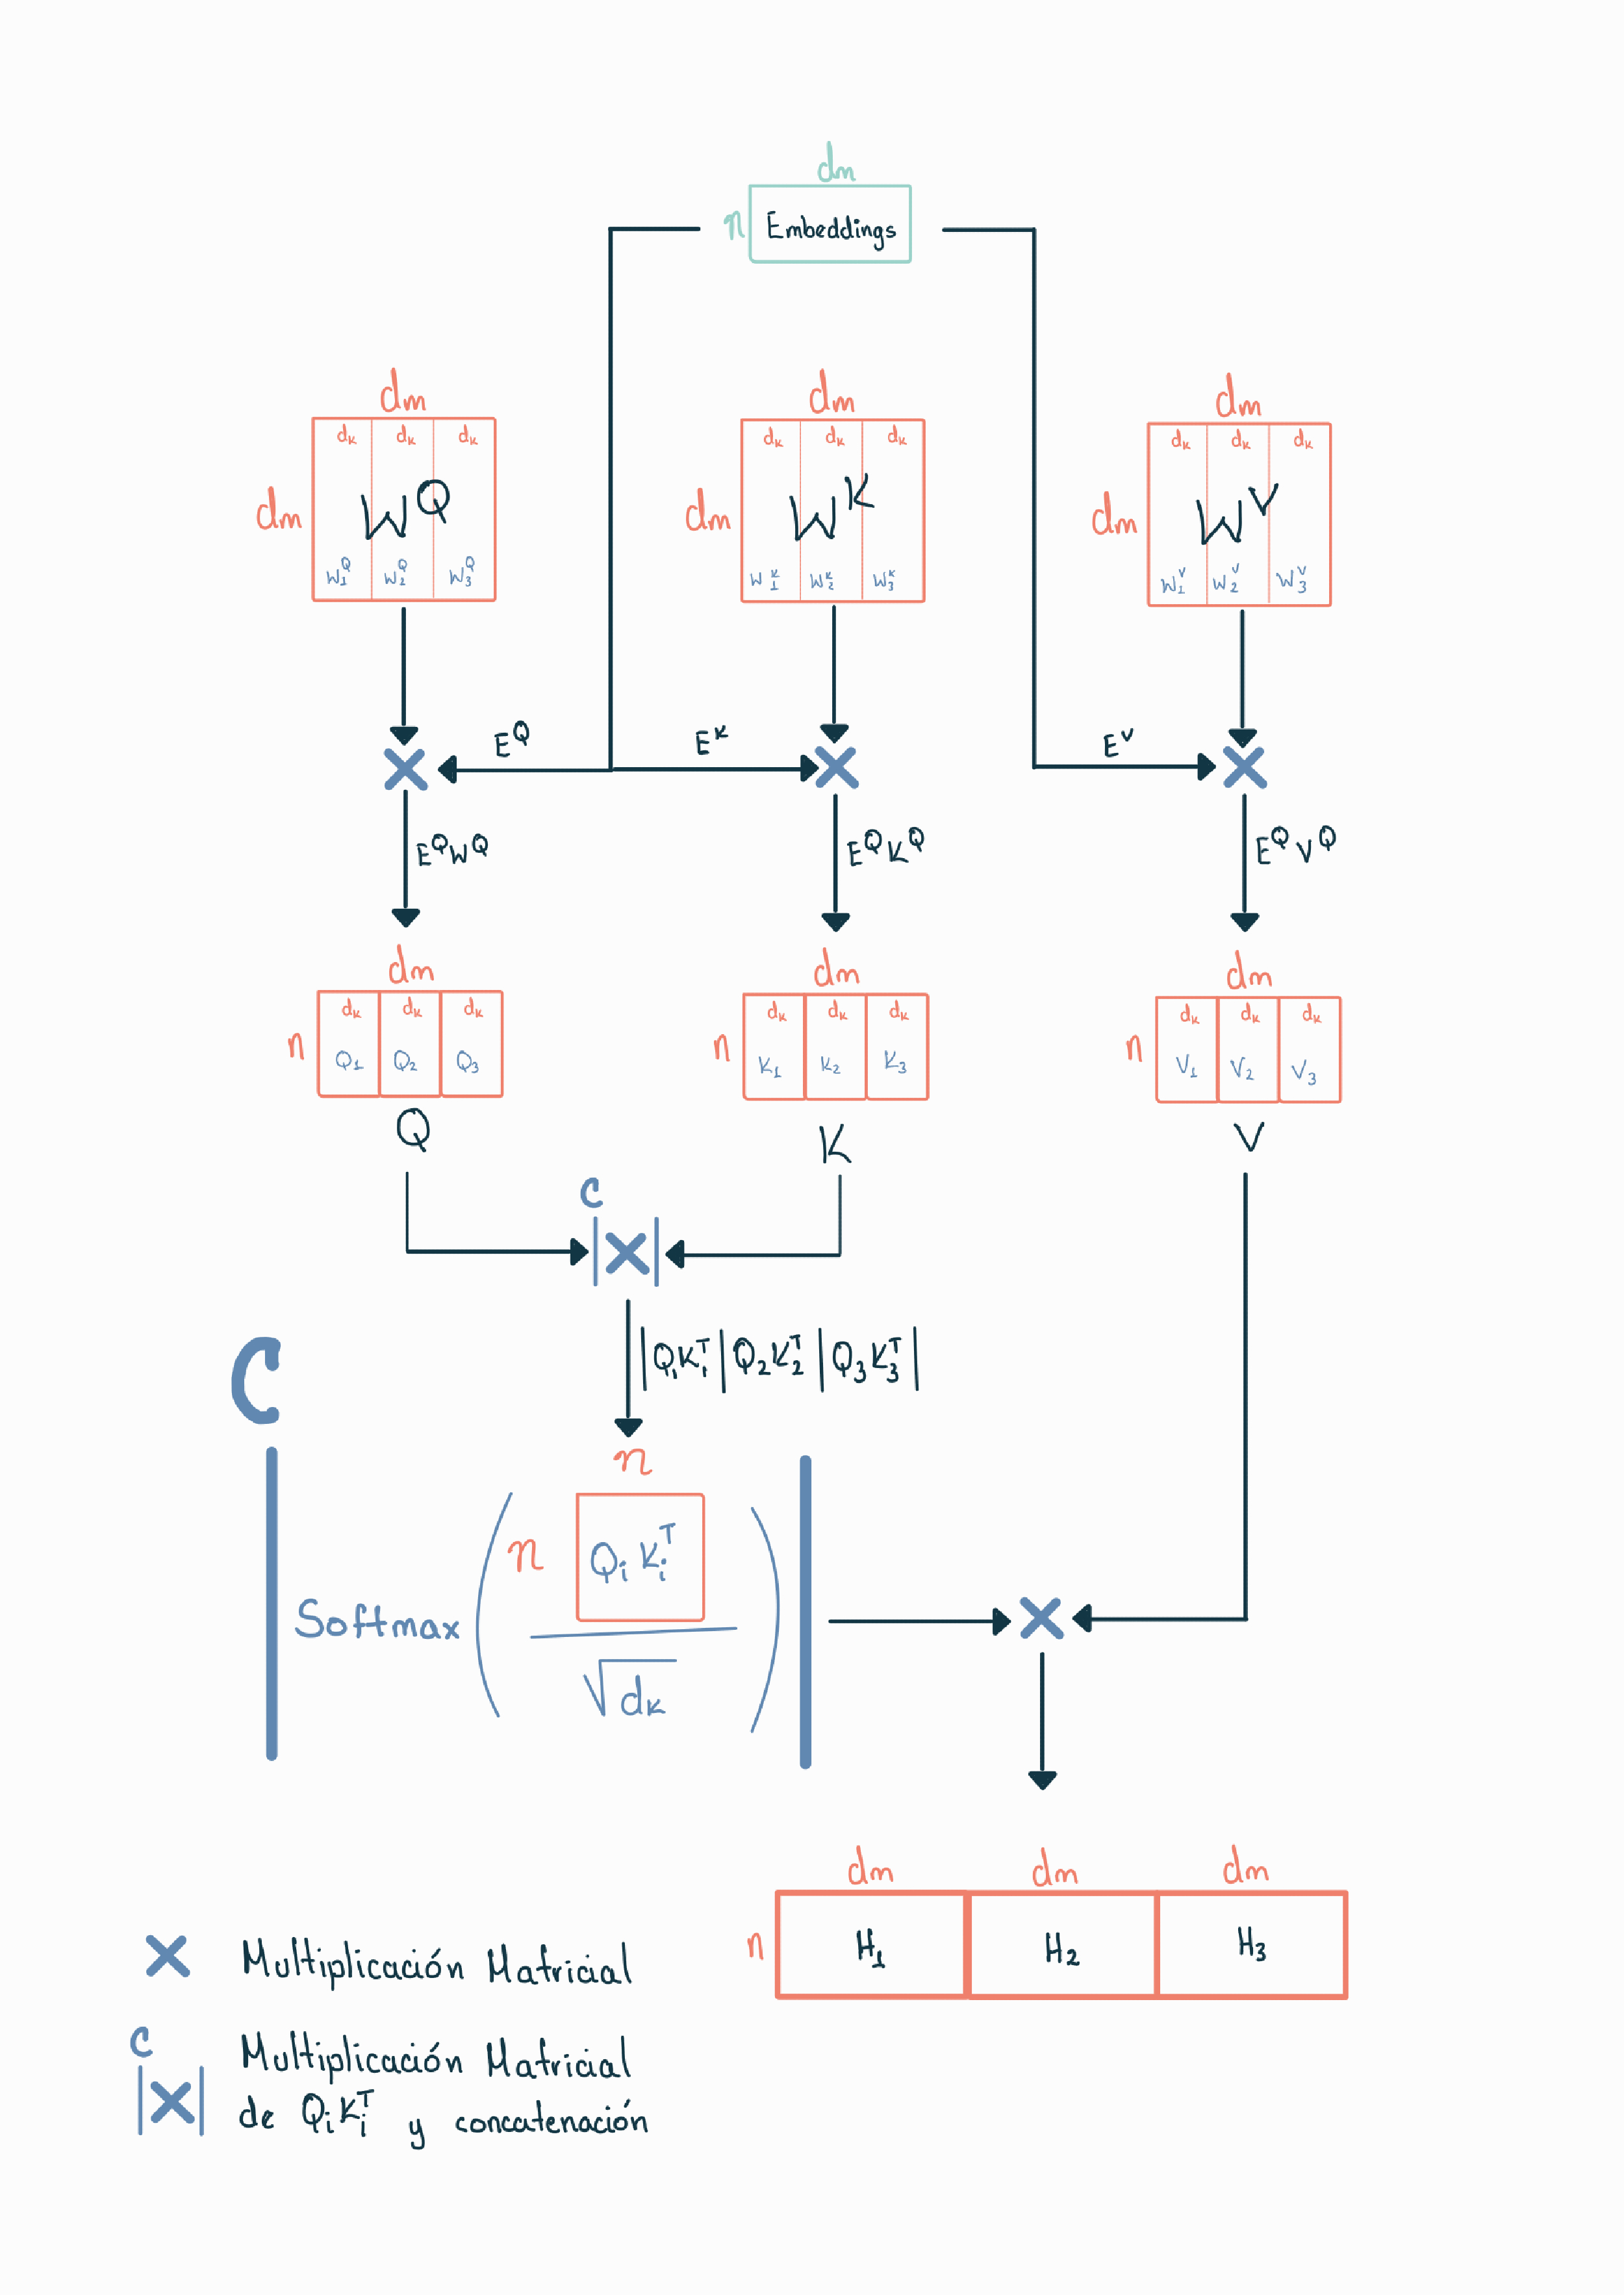
\includegraphics[width=0.7\textwidth]{../Chapters/4. ViT-Lung/images/cabezas_vit.jpg}
    \caption{Visualización de las cabezas de atención en el modelo ViT.}
\end{figure}
\end{frame}

\begin{frame}
\frametitle{Resumen de Resultados}
\begin{itemize}
    \item Ambos modelos superan o igualan el estado del arte en la mayoría de las patologías.
    \item El modelo ViT es especialmente competitivo en la detección de COVID-19.
    \item La arquitectura propuesta permite extender fácilmente la detección a nuevas patologías.
\end{itemize}
\end{frame}
